% Options for packages loaded elsewhere
\PassOptionsToPackage{unicode}{hyperref}
\PassOptionsToPackage{hyphens}{url}
\PassOptionsToPackage{dvipsnames,svgnames,x11names}{xcolor}
%
\documentclass[
true
]{sn-jnl}

\usepackage{amsmath,amssymb}
\usepackage{iftex}
\ifPDFTeX
  \usepackage[T1]{fontenc}
  \usepackage[utf8]{inputenc}
  \usepackage{textcomp} % provide euro and other symbols
\else % if luatex or xetex
  \usepackage{unicode-math}
  \defaultfontfeatures{Scale=MatchLowercase}
  \defaultfontfeatures[\rmfamily]{Ligatures=TeX,Scale=1}
\fi
\usepackage{lmodern}
\ifPDFTeX\else  
    % xetex/luatex font selection
\fi
% Use upquote if available, for straight quotes in verbatim environments
\IfFileExists{upquote.sty}{\usepackage{upquote}}{}
\IfFileExists{microtype.sty}{% use microtype if available
  \usepackage[]{microtype}
  \UseMicrotypeSet[protrusion]{basicmath} % disable protrusion for tt fonts
}{}
\makeatletter
\@ifundefined{KOMAClassName}{% if non-KOMA class
  \IfFileExists{parskip.sty}{%
    \usepackage{parskip}
  }{% else
    \setlength{\parindent}{0pt}
    \setlength{\parskip}{6pt plus 2pt minus 1pt}}
}{% if KOMA class
  \KOMAoptions{parskip=half}}
\makeatother
\usepackage{xcolor}
\setlength{\emergencystretch}{3em} % prevent overfull lines
\setcounter{secnumdepth}{-\maxdimen} % remove section numbering
% Make \paragraph and \subparagraph free-standing
\makeatletter
\ifx\paragraph\undefined\else
  \let\oldparagraph\paragraph
  \renewcommand{\paragraph}{
    \@ifstar
      \xxxParagraphStar
      \xxxParagraphNoStar
  }
  \newcommand{\xxxParagraphStar}[1]{\oldparagraph*{#1}\mbox{}}
  \newcommand{\xxxParagraphNoStar}[1]{\oldparagraph{#1}\mbox{}}
\fi
\ifx\subparagraph\undefined\else
  \let\oldsubparagraph\subparagraph
  \renewcommand{\subparagraph}{
    \@ifstar
      \xxxSubParagraphStar
      \xxxSubParagraphNoStar
  }
  \newcommand{\xxxSubParagraphStar}[1]{\oldsubparagraph*{#1}\mbox{}}
  \newcommand{\xxxSubParagraphNoStar}[1]{\oldsubparagraph{#1}\mbox{}}
\fi
\makeatother


\providecommand{\tightlist}{%
  \setlength{\itemsep}{0pt}\setlength{\parskip}{0pt}}\usepackage{longtable,booktabs,array}
\usepackage{calc} % for calculating minipage widths
% Correct order of tables after \paragraph or \subparagraph
\usepackage{etoolbox}
\makeatletter
\patchcmd\longtable{\par}{\if@noskipsec\mbox{}\fi\par}{}{}
\makeatother
% Allow footnotes in longtable head/foot
\IfFileExists{footnotehyper.sty}{\usepackage{footnotehyper}}{\usepackage{footnote}}
\makesavenoteenv{longtable}
\usepackage{graphicx}
\makeatletter
\newsavebox\pandoc@box
\newcommand*\pandocbounded[1]{% scales image to fit in text height/width
  \sbox\pandoc@box{#1}%
  \Gscale@div\@tempa{\textheight}{\dimexpr\ht\pandoc@box+\dp\pandoc@box\relax}%
  \Gscale@div\@tempb{\linewidth}{\wd\pandoc@box}%
  \ifdim\@tempb\p@<\@tempa\p@\let\@tempa\@tempb\fi% select the smaller of both
  \ifdim\@tempa\p@<\p@\scalebox{\@tempa}{\usebox\pandoc@box}%
  \else\usebox{\pandoc@box}%
  \fi%
}
% Set default figure placement to htbp
\def\fps@figure{htbp}
\makeatother

%%%% Standard Packages

\usepackage{graphicx}%
\usepackage{multirow}%
\usepackage{amsmath,amssymb,amsfonts}%
\usepackage{amsthm}%
\usepackage{mathrsfs}%
\usepackage[title]{appendix}%
\usepackage{xcolor}%
\usepackage{textcomp}%
\usepackage{manyfoot}%
\usepackage{booktabs}%
\usepackage{algorithm}%
\usepackage{algorithmicx}%
\usepackage{algpseudocode}%
\usepackage{listings}%

%%%%

\raggedbottom
\usepackage{booktabs}
\usepackage{longtable}
\usepackage{array}
\usepackage{multirow}
\usepackage{wrapfig}
\usepackage{float}
\usepackage{colortbl}
\usepackage{pdflscape}
\usepackage{tabu}
\usepackage{threeparttable}
\usepackage{threeparttablex}
\usepackage[normalem]{ulem}
\usepackage{makecell}
\usepackage{xcolor}
\makeatletter
\@ifpackageloaded{caption}{}{\usepackage{caption}}
\AtBeginDocument{%
\ifdefined\contentsname
  \renewcommand*\contentsname{Table of contents}
\else
  \newcommand\contentsname{Table of contents}
\fi
\ifdefined\listfigurename
  \renewcommand*\listfigurename{List of Figures}
\else
  \newcommand\listfigurename{List of Figures}
\fi
\ifdefined\listtablename
  \renewcommand*\listtablename{List of Tables}
\else
  \newcommand\listtablename{List of Tables}
\fi
\ifdefined\figurename
  \renewcommand*\figurename{\textbf{Figure}}
\else
  \newcommand\figurename{\textbf{Figure}}
\fi
\ifdefined\tablename
  \renewcommand*\tablename{\textbf{Table}}
\else
  \newcommand\tablename{\textbf{Table}}
\fi
}
\@ifpackageloaded{float}{}{\usepackage{float}}
\floatstyle{ruled}
\@ifundefined{c@chapter}{\newfloat{codelisting}{h}{lop}}{\newfloat{codelisting}{h}{lop}[chapter]}
\floatname{codelisting}{Listing}
\newcommand*\listoflistings{\listof{codelisting}{List of Listings}}
\captionsetup{labelsep=period}
\makeatother
\makeatletter
\makeatother
\makeatletter
\@ifpackageloaded{caption}{}{\usepackage{caption}}
\@ifpackageloaded{subcaption}{}{\usepackage{subcaption}}
\makeatother

\usepackage[]{natbib}
\bibliographystyle{plainnat}
\usepackage{bookmark}

\IfFileExists{xurl.sty}{\usepackage{xurl}}{} % add URL line breaks if available
\urlstyle{same} % disable monospaced font for URLs
\hypersetup{
  pdftitle={The Application of Magnetic Susceptibility Separation for Measuring Cerebral Oxygenation in Preterm Neonates},
  pdfauthor={, , , and },
  pdfkeywords={Quantitative Susceptbility
Mapping, Preterm, Newborn, Cerebral Venous Oxygen Saturation},
  colorlinks=true,
  linkcolor={blue},
  filecolor={Maroon},
  citecolor={Blue},
  urlcolor={Blue},
  pdfcreator={LaTeX via pandoc}}


\title[The Application of Magnetic Susceptibility Separation for
Measuring Cerebral Oxygenation in Preterm Neonates]{The Application of
Magnetic Susceptibility Separation for Measuring Cerebral Oxygenation in
Preterm Neonates}

% author setup
\author[1,2]{\fnm{Thomas Gavin} \sur{Carmichael}}\email{tgcarmichael@outlook.com}\author[3]{\fnm{Alexander} \sur{Rauscher}}\email{rauscher@physics.ubc.ca}\author[2,3]{\fnm{Ruth E} \sur{Grunau}}\email{rgrunau@mail.ubc.ca}\author*[2,3]{\fnm{Alexander Mark} \sur{Weber}}\email{aweber@bcchr.ca}
% affil setup
\affil[1]{, \orgname{Integrated Sciences, The University of British
Columbia, Vancouver, BC, Canada}}
\affil[2]{, \orgname{BC Children's Hospital Research Institute, The
University of British Columbia, Vancouver, BC, Canada}}
\affil[3]{, \orgname{Pediatrics, The University of British Columbia,
Vancouver, BC, Canada}}
\affil[4]{, \orgname{Physics and Astronomy, The University of British
Columbia, Vancouver, BC, Canada}}

% abstract 


% keywords
\keywords{Quantitative Susceptbility
Mapping,  Preterm,  Newborn,  Cerebral Venous Oxygen Saturation}

\begin{document}
\maketitle


\textsuperscript{1} Integrated Sciences, The University of British
Columbia, Vancouver, BC, Canada\\
\textsuperscript{2} BC Children's Hospital Research Institute, The
University of British Columbia, Vancouver, BC, Canada\\
\textsuperscript{3} Pediatrics, The University of British Columbia,
Vancouver, BC, Canada\\
\textsuperscript{4} Physics and Astronomy, The University of British
Columbia, Vancouver, BC, Canada

\textsuperscript{*} Correspondence:
\href{mailto:aweber@bcchr.ca}{Alexander Mark Weber
\textless{}aweber@bcchr.ca\textgreater{}}

\subsection{Impact Statement}\label{impact-statement}

\begin{itemize}
\tightlist
\item
  This study evaluated the use of QSM and its paramagnetic components to
  measure cerebral oxygenation in neonates.
\item
  By comparing susceptibility-derived oxygen saturation
  (SvO\textsubscript{2}) in the superior sagittal sinus (SSS) and
  central cerebral veins (CCV), it adds to the field of neonatal
  cerebral oxygenation measurement.
\item
  Decomposing QSM into paramagnetic components shows potential for
  improving SvO\textsubscript{2} accuracy, particularly in the SSS,
  though variability remains a challenge.
\item
  The results suggest no significant oxygenation difference between the
  SSS and CCV, contrasting with previous findings, indicating a need for
  further research on neonatal venous oxygenation.
\end{itemize}

\textbf{Category of Study:} basic science

\newpage{}

\subsection{Abstract:}\label{abstract}

\textbf{Background}: Quantitative susceptibility mapping (QSM), a
magnetic resonance imaging (MRI) modality sensitive to deoxyhemoglobin,
is a promising method for measuring cerebral oxygenation in human
neonates. Paramagnetic sources, like deoxyhemoglobin, however, can be
obscured by diamagnetic sources such as water and myelin. This study
evaluated whether QSM images, or isolated paramagnetic components, are
more accurate for measuring oxygenation of cerebral veins of preterm
neonates, and explored oxygenation differences between the major
cerebral veins.

\textbf{Methods}: 19 preterm neonates were scanned on at term equivalent
age on a 3T MRI using a multi-echo susceptibility-weighted imaging
sequence. Susceptibility values were calculated from QSM images to
determine oxygen saturation (SvO\textsubscript{2}) in the superior
sagittal sinus (SSS) and central cerebral veins (CCV). The paramagnetic
components of QSM images were isolated, and SvO\textsubscript{2} values
were recalculated.

\textbf{Results}: The mean SvO\textsubscript{2} values from QSM were
72.4\% (SD, 3.4\%) for the SSS and and 68.7\% (SD, 3.5\%) for the CCV.
SvO\textsubscript{2} values for paramagnetic components were 58.1\% (SD,
7.3\%) for the SSS and 57.7\% (SD, 7.0\%) for the CCV.

\textbf{Conclusion}: While paramagnetic component decomposition yielded
SSS values closer to those found in the literature, it increased
variability. No significant oxygenation differences were found between
the SSS and CCV, contrasting with prior studies.

\textsubscript{Source:
\href{https://WeberLab.github.io/Chisep_CSVO2_Manuscript/index.qmd.html}{Article
Notebook}}

\textsubscript{Source:
\href{https://WeberLab.github.io/Chisep_CSVO2_Manuscript/index.qmd.html}{Article
Notebook}}

\textsubscript{Source:
\href{https://WeberLab.github.io/Chisep_CSVO2_Manuscript/index.qmd.html}{Article
Notebook}}

\newpage{}

\section{Introduction}\label{sec-intro}

With advances in neonatal medical care, more infants born preterm are
surviving into childhood \citep{mckenzieScaffoldingParentingHealth2022}.
These children are at high risk of acquiring adverse neurodevelopmental
outcomes when compared to their term-born peers
\citep{twilhaarCognitiveOutcomesChildren2018}. Irregularities in early
cerebral oxygen levels have been identified as a potential source of
such delays, where too little oxygen provided during NICU care can
result in white matter injury, while too much oxygen can result in
reduced cortical connectivity \citep{rantakariEarlyOxygenLevels2021}. As
such, being able to precisely, accurately, and non-invasively measure
cerebral oxygenation is necessary for understanding and improving
neurodevelopmental outcomes in preterm neonates.

Unfortunately, there exist many challenges in measuring cerebral oxygen
metabolism in neonates. Cerebral metabolic rate of oxygen
(CMRO\textsubscript{2}) using oxygen-15 positron emission tomography
(PET) \citep{mintunBrainOxygenUtilization1984}, has been measured in
infants \citep{altmanCerebralBloodFlow1988}, and is considered the gold
standard. However, this method is invasive, requiring ionizing
radiation, which limits its suitability for neonates. A less invasive
option for evaluating brain hemodynamics is near-infrared spectroscopy
(NIRS), which uses the attenuation of near-infrared light
(\textasciitilde650--950 nm) as it passes through biological tissue
\citep{skovEstimationCerebralVenous1993}. Deoxygenated and oxygenated
hemoglobin absorb this light differently, allowing NIRS to estimate
changes in deoxyhemoglobin and oxyhemoglobin
\citep{wrayCharacterizationInfraredAbsorption1988} and thus provide an
estimate of cerebral venous oxygen saturation (SvO\textsubscript{2}).
While NIRS offers the advantage of being non-invasive and continuous
bedside monitoring, it is limited to regional assessments where the
probe is placed and is sensitive only to superficial brain tissue due to
the shallow penetration depth of near-infrared light
\citep{boasDiffuseOpticalImaging2004}.

For the preceding reasons, non-invasive MRI-based techniques are
actively being explored to assess regional and whole-brain blood
oxygenation. While MRI-based methods have been developed for adults
\citep{jainRapidMagneticResonance2011, luQuantitativeEvaluationOxygenation2008, xuNoninvasiveQuantificationWholebrain2009},
their application in neonates is only beginning to be explored
\citep{devisNoninvasiveMRIMeasurements2014, liuQuantitativeAssessmentGlobal2014, qiHemodynamicMetabolicAssessment2018, jainCerebralOxygenMetabolism2014, jiangVesselspecificQuantificationNeonatal2019}.
This delay is likely due to the unique challenges posed by neonates,
including their smaller anatomies, distinct hemodynamic profiles,
susceptibility to motion artifacts, and the difficulties associated with
recruiting this population for research. These methods have almost all
relied on T2 relaxation to estimate CSvO\textsubscript{2}
\citep{devisNoninvasiveMRIMeasurements2014, liuQuantitativeAssessmentGlobal2014, qiHemodynamicMetabolicAssessment2018, jiangVesselspecificQuantificationNeonatal2019}
with the exception of \citet{jainCerebralOxygenMetabolism2014} which
used susceptometry \citep{jainMRIEstimationGlobal2010}. One limitation
of these T2 relaxation methods, however, is the fact that
SvO\textsubscript{2} is often measured using a single imaging slice,
averaging values across several voxels, and only in the superior
sagittal sinus (SSS). In the case of
\citet{jainCerebralOxygenMetabolism2014}, they obtained regional and
whole-brain data, but with thick slices (5mm), and still only estimated
CSvO\textsubscript{2} in the SSS. An alternative MRI method using
quantitative susceptibility mapping (QSM) has been proposed, which can
measure SvO\textsubscript{2} regionally and across the whole-brain at
high resolution (\textless{} 1mm\textsuperscript{3} per voxel)
\citep{weberQuantitativeSusceptibilityMapping2021}. However, this method
left room for improvement, as it removed the SSS (averaging
CSvO\textsubscript{2} across the internal veins), and required an
arbitrary threshold value of 0.15 ppm in order to acquire realistic
results \citep{weberQuantitativeSusceptibilityMapping2021}. Furthermore,
QSM tends to underestimates parametric components due to the inclusion
of diamagnetic tissue, and vice versa, as the opposing magnetic
susceptibilities effectively subtract from one another
\citep{kimHSeparationImagingDiagnosis2023}.

In the present study, we set out to determine whether decomposing the
QSM image into its paramagnetic and diamagnetic components would allow
for a more accurate assessment of SvO\textsubscript{2} in the central
cerebral veins (CCV) of a cohort of preterm neonates. We also had a
secondary aim of preserving the SSS vessel in our QSM images and using
this data to determine whether a difference in oxygenation existed
between the SSS and the CCV.

\section{Methods}\label{sec-data-methods}

The study was approved by the Clinical Research Ethics Board at the
University of British Columbia and Children's \& Women's Hospital
(H21-00655) and written informed consent was obtained from the
parent/guardian for each infant.

\subsection{Study population}\label{study-population}

Participant data comes from a previous study *** . Participants
consisted of preterm neonates born between 25- and 31-weeks gestational
age (GA) who were admitted to the level III NICU at *** . Recruitment
took place over a span of one year, from February 2021 to January 2022,
facilitated by a dedicated research nurse. Parents of eligible infants
were approached by the research nurse prior to discharge from the NICU
to explain the study objectives and seek their consent for
participation. Infants meeting the criteria for inclusion were scanned
for the study if they had already been discharged from the NICU, were in
stable condition, and had reached a term equivalent age of 37 to 44
weeks GA. However, certain exclusion criteria were applied to ensure the
homogeneity and integrity of the study sample: infants were excluded if
there was clinical evidence of a congenital malformation or syndrome, a
TORCH infection, or ultrasound evidence of large parenchymal hemorrhagic
infarction (\textgreater2 cm, Grade 4 intraventricular hemorrhage).

\subsection{Image acquisition}\label{image-acquisition}

MR imaging was performed on a 3.0 Tesla General Electric Discovery MR750
scanner (scanner software version DV26.0\_R03) equipped with a SREE
Medical Systems (Cleveland, OH) single-channel neonatal head coil
(Table~\ref{tbl-mri}). The scans were conducted at the *** 's MRI
Research Facility. Prior to the scanning procedure, subjects were
carefully prepared by a research nurse. Swaddling and feeding were used
to ensure the comfort and cooperation of the subjects during the scan.
Importantly, no sedatives or invasive markers were utilized throughout
the procedure. Subjects were placed within a specially designed SREE
Medical Systems MRI compatible incubator, which facilitated both safety
and motion minimization. Molded foam was strategically positioned around
the head and body within the incubator to further restrict subject
movement. To protect against potential hearing damage, ear plugs were
employed during the scanning process. Additionally, a pulse oximeter was
affixed to the subject's foot to monitor arterial oxygen saturation and
heart rate throughout the scan.

\begingroup\fontsize{8}{10}\selectfont

\begin{ThreePartTable}
\begin{TableNotes}[para]
\item T1w = T1-weighted; T2w = T2-weighted; pcASL = pseudo-continuous arterial spin labelling; SWI = susceptibility weighted imaging; FSPG = fast spoiled gradient echo; CUBE = General Electric name of sequence, not an acronym; GRE = gradient echo; ZIP2 = through-plane zero filling interpolation
\end{TableNotes}

\begin{longtable}[t]{>{\raggedright\arraybackslash}p{8em}ll>{\raggedright\arraybackslash}p{9em}>{\raggedright\arraybackslash}p{9em}}

\caption{\label{tbl-mri}\textbf{Technical parameters for MR imaging
pulse sequences}}

\tabularnewline

\toprule
 & \textbf{T1w} & \textbf{T2w} & \textbf{pcASL} & \textbf{SWI}\\
\midrule
Sequence & 3D FSPGR & 3D CUBE & Multi-shot 3D fast spin-echo & 3D spoiled GRE flow-compensated\\
Acquisition plane & Coronal & Sagittal & Axial & Axial\\
Phase-encoding direction & Left-Right & Posterior-Anterior & Posterior-Anterior & Left-Right\\
TR (ms) & 7.74 & 2,300 & 4,680 & 30.9\\
TE (ms) & 2.97 & 66.29 & 10.55 & 5 echoes; first echo: 5; echo spacing: 5.24\\
Flip angle & 12° & 90° & 111° & 20°\\
FOV (cm) & 20 & 20 & 24 & 25\\
Acquisition matrix & 512 x 512 & 256 x 256 & 128 x 128 & 256 x 256\\
In-plane resolution (mm) & 0.39 x 0.39 & 0.78 x 0.78 & 1.875 x 1.875 & 0.977 x 0.977\\
Slice thickness (mm) & 1 & 1 & 4 & 2, reconstructed to 1 with zero filling (ZIP2)\\
Number of slices & 126 & 106 & 50 & 92\\
Additional parameters & n/a & n/a & 1,450 ms label period;\newline  2,025 ms pulse label;\newline  24 control-label pairs & n/a\\
Scan duration & 4 min 39 s & 5 min 1 s & 5 min 26 s & 5 min 29 s\\
\bottomrule
\insertTableNotes

\end{longtable}

\end{ThreePartTable}
\endgroup{}

\textsubscript{Source:
\href{https://WeberLab.github.io/Chisep_CSVO2_Manuscript/index.qmd.html}{Article
Notebook}}

The MRI scan protocol comprised of the following sequences (plane of
acquisition in parentheses): a T1-weighted scan (coronal), a T2-weighted
scan (sagittal), a pseudo-continuous arterial spin labeling (ASL) scan
\citep{alsopRecommendedImplementationArterial2015} (axial), a multi-echo
susceptibility-weighted imaging scan
\citep{denkSusceptibilityWeightedImaging2010} (axial), and a
diffusion-weighted imaging (DWI) spin-echo echo planar imaging (EPI)
sequence (axial). The DWI sequence was not used for the present study.

\subsection{Image analysis}\label{image-analysis}

The raw DICOM files acquired from the scanning procedure were converted
to NIfTI (Neuroimaging Informatics Technology Initiative) format using
Chris Rorden's \texttt{dcmniix} tool
\citep{liFirstStepNeuroimaging2016}. SWI magnitude data files were then
used to create subject-specific brain masks that would not erode the SSS
during QSM processing, an issue faced by our group in the past *** . A
step-by-step summary of the pipeline used is shown in
Figure~\ref{fig-graph}.

\begin{figure}[H]

\centering{

\pandocbounded{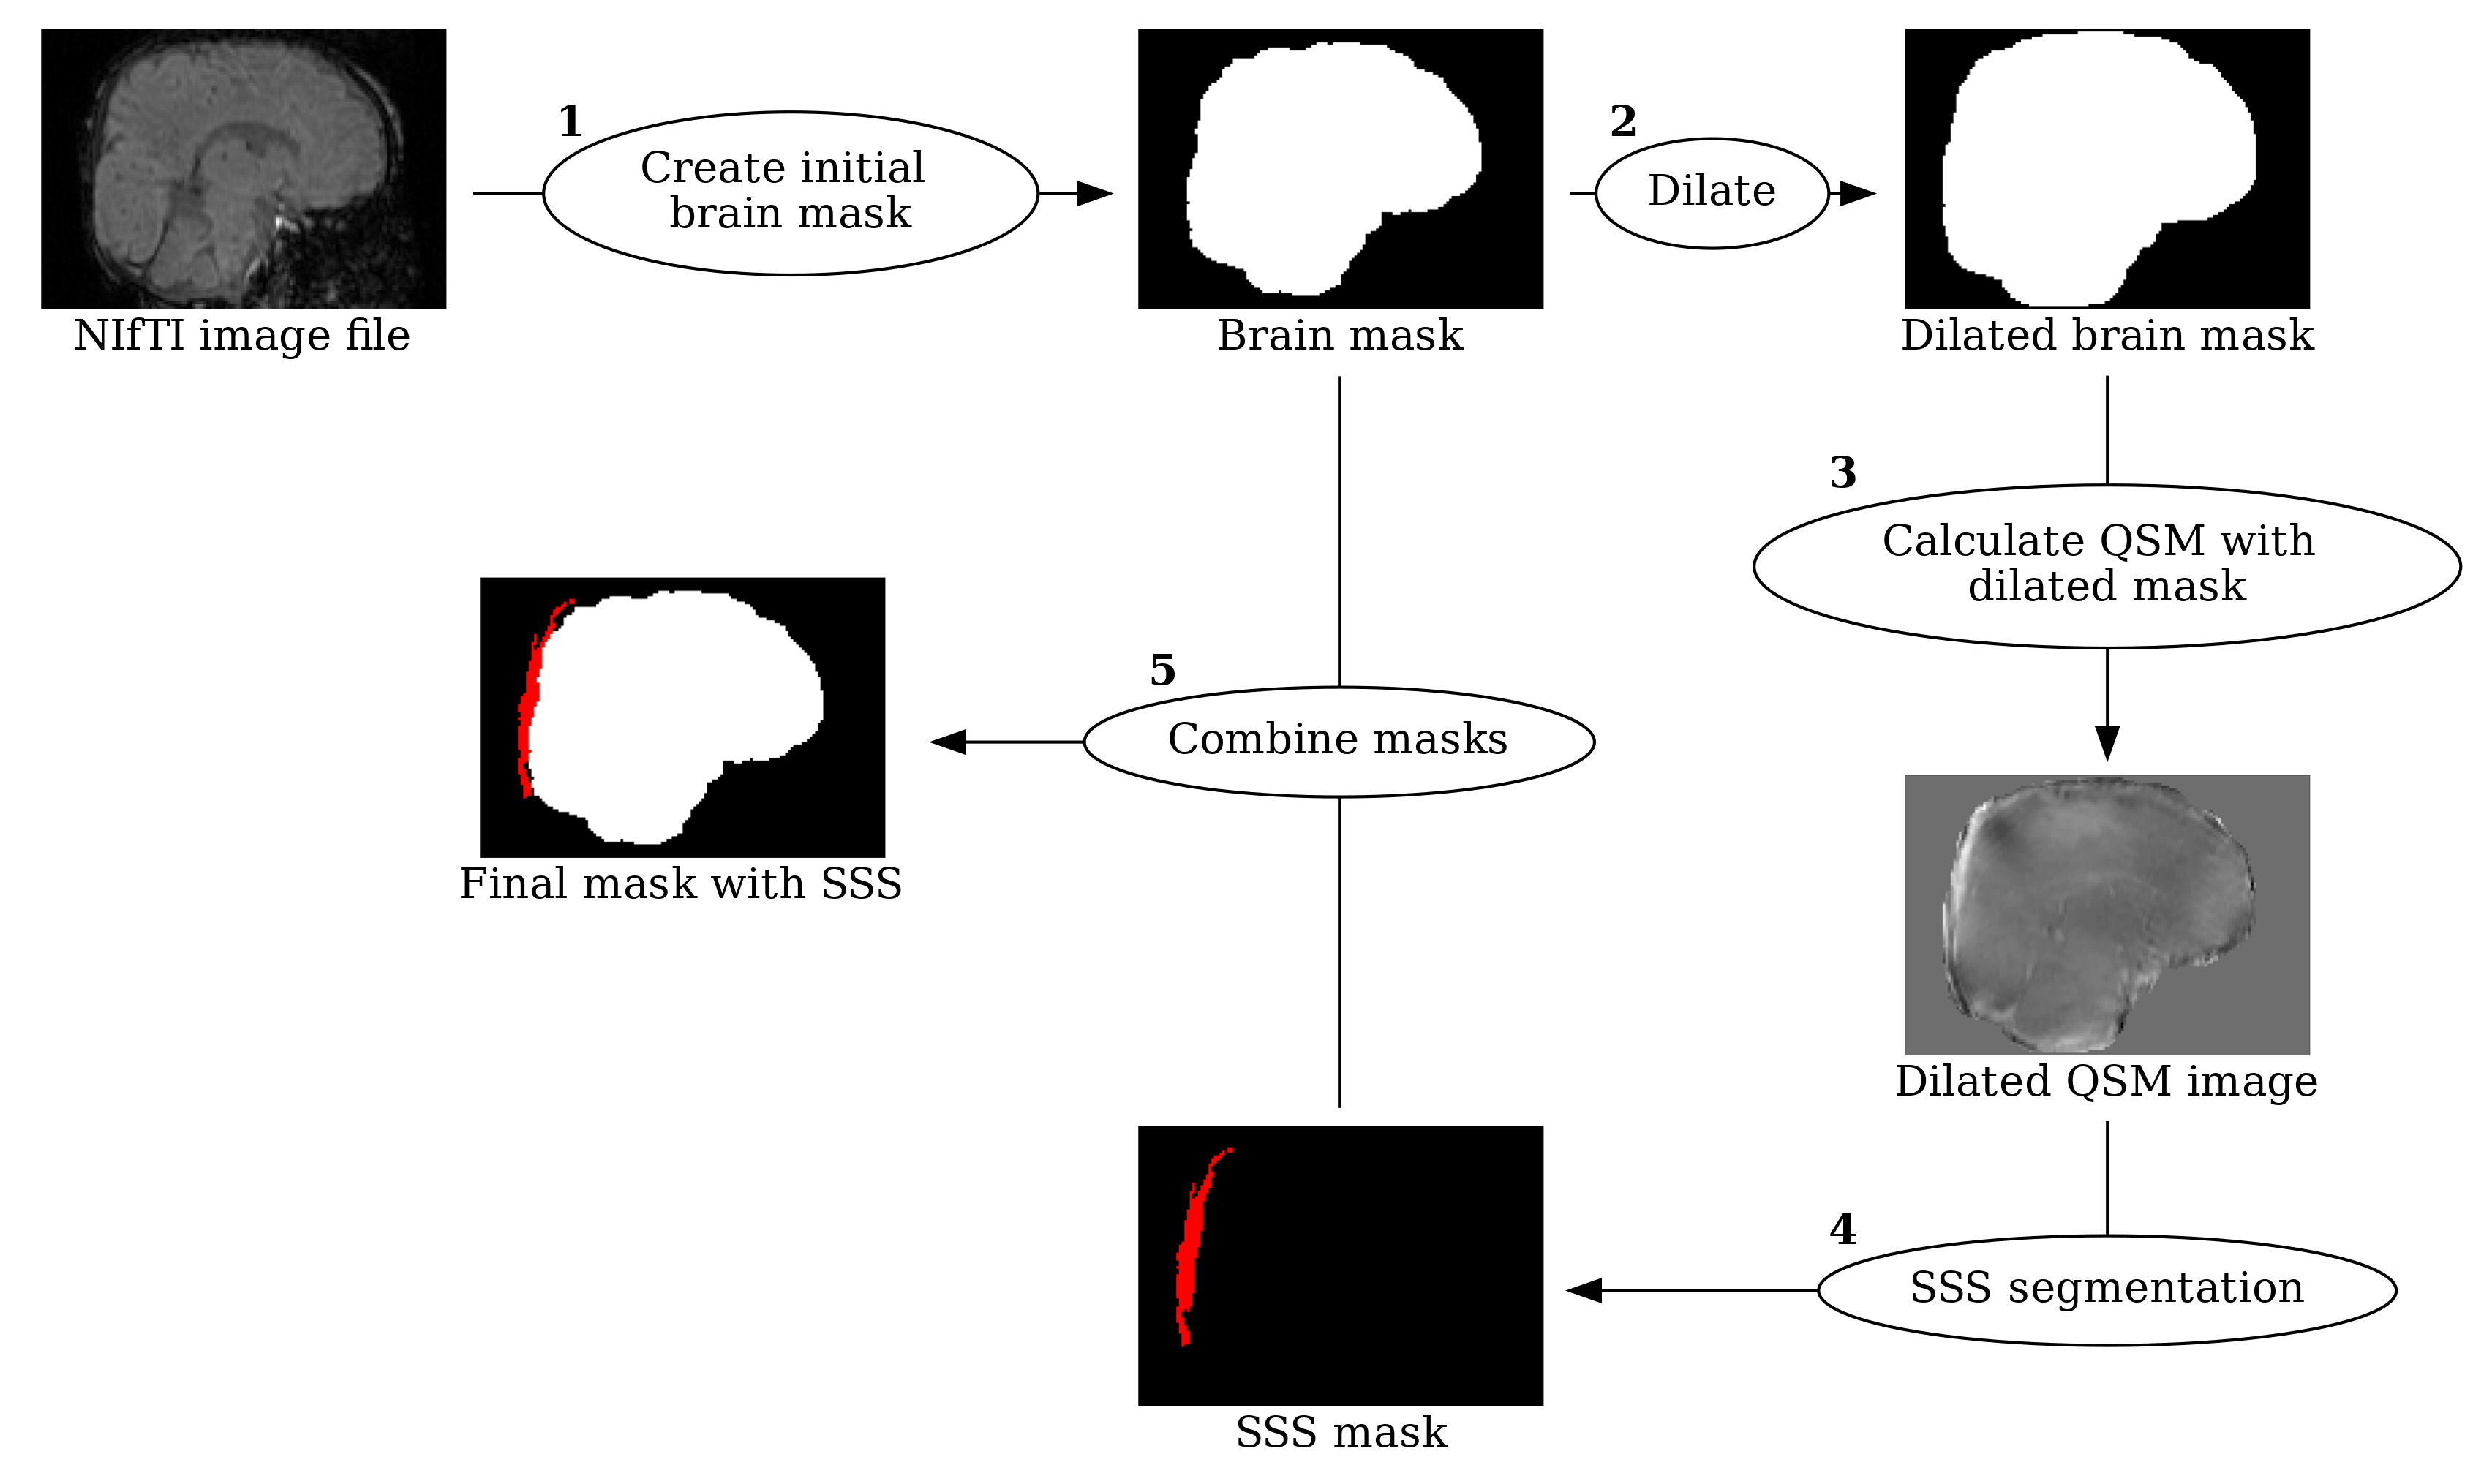
\includegraphics[keepaspectratio]{index_files/figure-latex/notebooks-Figures-fig-graph-output-1.png}}

}

\caption{\label{fig-graph}\textbf{Pipeline for generating
subject-specific brain masks that include the superior sagittal sinus
(SSS).} Initial steps involved (1) creating brain a mask from the
magnitude of the fifth echo of the susceptibility weighted scan.
Subsequently, the brain mask is dilated and then (2) utilized in
conjunction with a quantitative susceptibility mapping (QSM) script to
generate a preliminary QSM image. Further refinement involved (3)
segmenting the SSS from the QSM image manually to create a tissue mask
of the SSS region. Finally, (4) the vascular mask of the SSS is
integrated with the initial brain mask, forming the comprehensive brain
mask essential for obtaining susceptibility data that includes the SSS.}

\end{figure}%

\textsubscript{Source:
\href{https://WeberLab.github.io/Chisep_CSVO2_Manuscript/notebooks/Figures-preview.html\#cell-fig-graph}{Python
Figures}}

First, the fifth echo (TE = 25.96 ms) SWI magnitude file was processed
using FSL's (v. 6.0.7.3)
\citep{woolrichBayesianAnalysisNeuroimaging2009} \texttt{fslroi},
\texttt{fslmaths}, and \texttt{bet} \citep{smithFastRobustAutomated2002}
to create a preliminary brain mask, similar to our previous efforts,
which does not contain the SSS. The last echo is used to generate the
brain mask as it reliably removes artifacts from air-tissue and
bone-tissue interfaces, e.g., sinuses, without the need for manual
erosion. The reason for this is at longer echo times, tissues with rapid
signal decay (such as bone, air, and sinuses) lose their MRI signal due
to dephasing caused by greater magnetic field inhomogeneities.
\texttt{Fslroi} was used to isolate the fifth echo of the magnitude
data, which was then squared using \texttt{fslmaths} and the option
\texttt{-sqr}. Squaring the magnitude image was found to dramatically
improve subsequent brain extraction. The resulting image was then used
to create the preliminary brain mask using \texttt{bet} with the options
\texttt{-m} and \texttt{-R}. The former flag generated a binary brain
mask, while the latter performed a more robust brain centre estimation.
The brain mask was then dilated by 7 voxels using \texttt{fslmaths} and
the options \texttt{-kernel\ boxv} and \texttt{-dilM} in order for the
dilated mask to contain the SSS (along with unwanted tissue as well).
This mask was then used, along with the phase images, in a MATLAB script
for QSM calculation from Christian Kames
\citep{kamesRapidTwostepDipole2018} to produce a preliminary QSM image
that contained the SSS, albeit with fairly low signal-to-noise ratio and
other unwanted tissue. Given the high contrast in voxel intensity
between the SSS and surrounding tissue, the select by intensity tool in
\texttt{FSLeyes} \citep{mccarthyFSLeyes2023} was then used to segment
the SSS from the QSM image and create a 3D mask of the selected region.
Using \texttt{fslmaths} and the options \texttt{-add} and \texttt{-bin},
the SSS mask was then combined with the original brain mask of the fifth
echo. This resulted in a brain mask that contained only brain and SSS
signal. Finally, this mask was used in a final QSM post-processing step
to create a QSM image that includes the SSS while maintaining a high
signal-to-noise ratio, making it suitable to obtain accurate
susceptibility values.

STI Suite (v. 3.0) \citep{liIntegratedLaplacianbasedPhase2014}, was used
to process the final QSM images as it produced the images with the least
amount of artifacts (based on a visual assessment by the authors)
without eroding the SSS. The finalized brain mask along with all five
echoes of the magnitude and phase images were used in STI Suite along
with the following parameters: 0.9766 x 0.9766 x 1 mm\textsuperscript{3}
voxel size, 5 ms TE1, 5.24 ms \(\Delta\)TE, and 77.4 ms sum TE, B0
strength = 3, and B0 direction = {[}0, 0, 1{]}. The 3D GRE data option
was selected for the phase processing stage, and STAR-QSM was selected
for the QSM stage. STAR-QSM outputs a single QSM map for each echo
(i.e.~five total). The last three echoes of the QSM maps were then
averaged to create the final QSM image using \texttt{fslmaths}, as the
accumulation of phase due to susceptibility is small in early echoes and
artifacts dominate the phase
\citep{zhangQuantitativeAnalysisPunctate2019}. Finally, the `select by
intensity' tool in \texttt{FSLeyes} was then used to semi-automatically
make vascular masks of the SSS and CCV from each subject's QSM image
(Figure~\ref{fig-masks}). The vascular masks were used to calculate the
mean susceptibility of each subject's SSS and CCV from their QSM image
with \texttt{fslstats}.

\begin{figure}[H]

\centering{

\pandocbounded{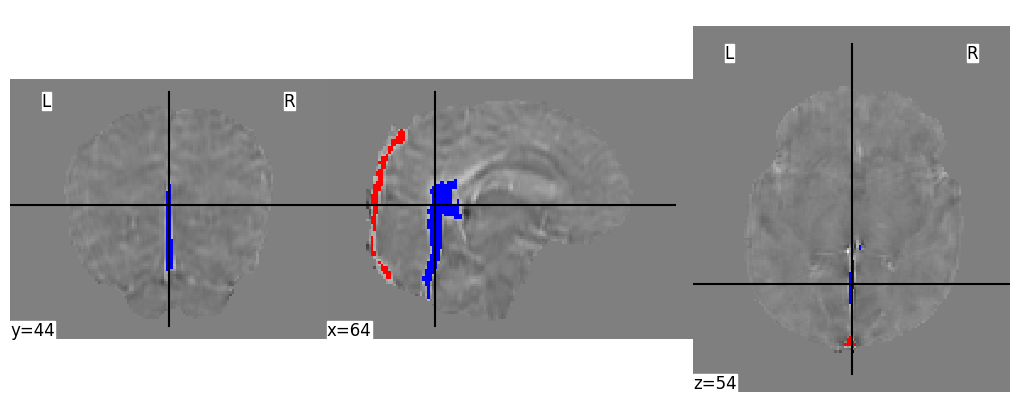
\includegraphics[keepaspectratio]{index_files/figure-latex/notebooks-Figures-fig-masks-output-1.png}}

}

\caption{\label{fig-masks}\textbf{Sample venous masks.} A sample
superior sagittal sinus (red) and central cerebral vein mask (blue)
displayed in coronal, sagittal, and axial view. The QSM image is used as
the underlay. y, x and z values represent the slice number in each plane
(coronal, sagittal, and axial, respectively).}

\end{figure}%

\textsubscript{Source:
\href{https://WeberLab.github.io/Chisep_CSVO2_Manuscript/notebooks/Figures-preview.html\#cell-fig-masks}{Python
Figures}}

To isolate the paramagnetic component of subjects' QSM data, the
\(\chi\)-separation toolbox
\citep{shinHseparationMagneticSusceptibility2021} from the Laboratory
for Imaging Science and Technology was used. All five echoes of each
subject's magnitude and phase SWI data were used along with the
following parameters: 0.9766 x 0.9766 x 1 mm\textsuperscript{3} voxel
size; TE (ms) = {[}5, 10.24, 15.48, 20.72, 26.96{]}; \(\Delta\)TE (ms) =
5.24; B0 strength = 3; B0 direction = {[}0, 0, 1{]}. The
\(\chi\)-separation toolbox outputs a single negative (diamagnetic),
positive (paramagnetic), and total \(\chi\) map (QSM). The mean
susceptibility of each subject's SSS and CCV in their paramagnetic maps
was calculated with the same vascular masks used for the QSM images.
Sample images showing the magnitude, final QSM, and final paramagnetic
component images are shown in Figure~\ref{fig-sample}.

\begin{figure}[H]

\centering{

\pandocbounded{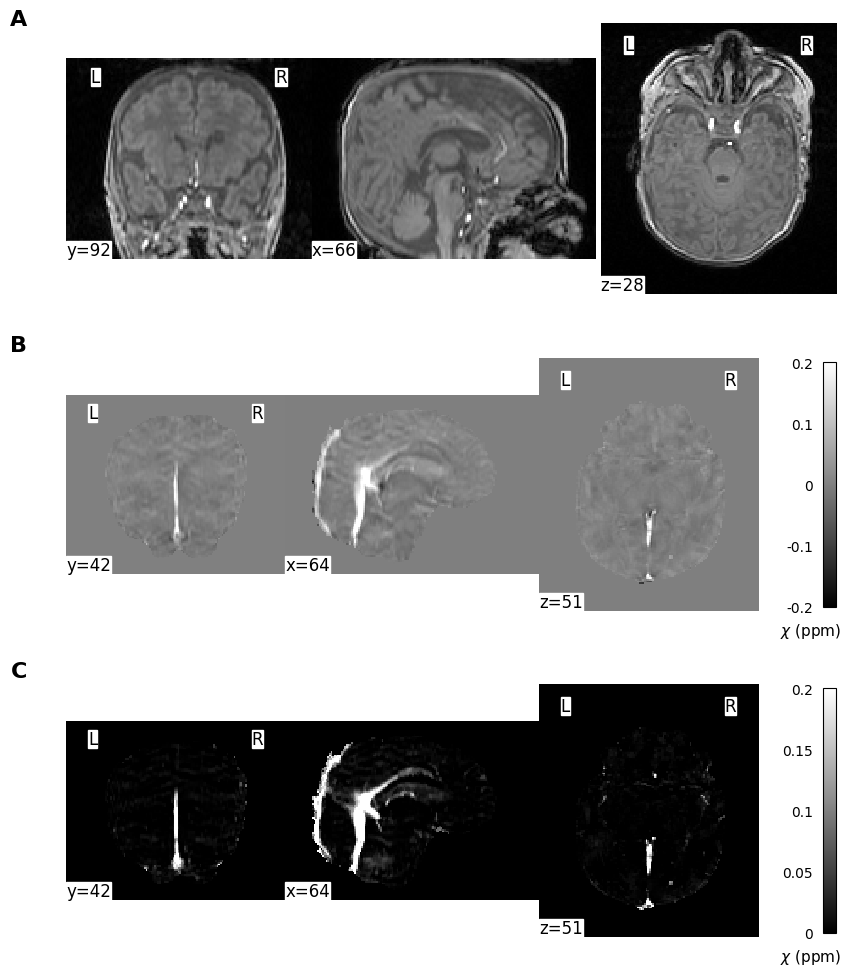
\includegraphics[keepaspectratio]{index_files/figure-latex/notebooks-Figures-fig-sample-output-1.png}}

}

\caption{\label{fig-sample}\textbf{An example of subject imaging data.}
A sample coronal, sagittal, and axial slice is displayed for each image.
(a) The 1st echo of the magnitude susceptibility weighted imaging
sequence; (b) the final quantitative susceptibility mapping image; and
(c) the paramagnetic component isolated from the quantitative
susceptibility map. The color bars in (b) and (c) indicates the range of
susceptibility \(\chi\) values in parts per million. y, x and z values
represent the slice number in each plane (coronal, sagittal, and axial,
respectively).}

\end{figure}%

\textsubscript{Source:
\href{https://WeberLab.github.io/Chisep_CSVO2_Manuscript/notebooks/Figures-preview.html\#cell-fig-sample}{Python
Figures}}

Once the mean susceptibility values of the SSS and CCV were obtained
from the subjects' QSM images or paramagnetic maps, venous oxygen
saturation (SvO\textsubscript{2}) was calculated with the following
equation \citep{bergInvestigatingEffectFlow2021}:

\begin{equation}\phantomsection\label{eq-svo}{
SvO_{2} = 1 - \frac{\Delta \chi _{blood} - (\Delta \chi _{oxy} * Hct)}{\Delta \chi _{do} * Hct}
}\end{equation}

where \(\Delta \chi _{blood}\) is the vessel's measured susceptibility,
\(\Delta \chi _{oxy}\) is the constant representing the susceptibility
changes of oxygenated blood relation to water, \(\Delta \chi _{do}\) is
the difference in susceptibility between oxygenated and deoxygenated
blood, and Hct is the subject's hematocrit. \(\Delta \chi _{oxy}\) was
-0.21 * 4\(\pi\) ppm as per \citet{portnoyHumanUmbilicalCord2018} and
\citep{sedlacikObtainingBloodOxygenation2007}, while
\(\Delta \chi _{do}\) was -0.03 * 4\(\pi\) ppm as per
\citep{weisskoffMRISusceptometryImagebased1992}. Subjects' Hct for the
day of the scan was calculated using a four-parameter Weibull function
with previously measured values while still in the NICU.

\subsection{Statistical analysis}\label{statistical-analysis}

Statistical analysis was performed using R and RStudio (v. 2023.09.1
Build 494)
\citep{rcoreteamLanguageEnvironmentStatistical2022, rstudioteamRStudioIntegratedDevelopment}.
Mean and standard deviation values are reported for most statistics,
unless specified otherwise. A paired Student's t-test was used to
determine statistical significance (p \textless0.05) between two
parameters (e.g.~\(\chi\) values between venous structures).

\section{Results}\label{sec-results}

A total sample size of 19 infants were scanned, with a mean (\(\pm\)
standard deviation) gestational age of 28.8 \(\pm\) 1.68 weeks and a
mean birth weight of 1276.05 \(\pm\) 294.87 grams. A comprehensive
summary of neonatal characteristics, including additional demographic
and clinical data, is provided in Table~\ref{tbl-dem} for reference.

\begingroup\fontsize{9}{11}\selectfont

\begin{ThreePartTable}
\begin{TableNotes}[para]
\item SD = standard deviation; IQR = inter quartile range
\end{TableNotes}

\begin{longtable}[t]{lr}

\caption{\label{tbl-dem}\textbf{Demographic and clinical characteristic
of the study sample.}}

\tabularnewline

\toprule
\textbf{Variable} & \textbf{Subject data (n=19)}\\
\midrule
Gestational age, weeks (mean ± SD) & 28.8 ± 1.68\\
Corrected gestational age on scan day, weeks (mean ± SD) & 40.36 ± 1.4\\
Number of male neonates (\%) & 10 (52.63)\\
Birth weight, g (mean ± SD) & 1276.05 ± 294.87\\
Weight on scan day, g (mean ± SD) & 3396.58 ± 597.72\\
Days spent in NICU (median, IQR) & 53, 23\\
Days on ventilation (median, IQR) & 31, 28.5\\
\bottomrule
\insertTableNotes

\end{longtable}

\end{ThreePartTable}
\endgroup{}

\textsubscript{Source:
\href{https://WeberLab.github.io/Chisep_CSVO2_Manuscript/index.qmd.html}{Article
Notebook}}

The mean SvO\textsubscript{2} values for the SSS and the CCV were found
to be 0.72 \(\pm\) 0.03\% and 0.69 \(\pm\) 0.03\%, respectively, when
determined from the QSM data. When determined from the paramagnetic map,
the mean SvO\textsubscript{2} values for the SSS and the CCV were found
to be 0.58 \(\pm\) 0.07\% and 0.58 \(\pm\) 0.07\%, respectively. A
summary of the measured physiological parameters, including the chi
values used to calculate SvO\textsubscript{2}, can found in
Table~\ref{tbl-chistats}.

\begingroup\fontsize{9}{11}\selectfont

\begin{ThreePartTable}
\begin{TableNotes}[para]
\item QSM = quantitative susceptibility mapping; CI = confidence interval; SSS = superior sagitall sinus; CCV = central cerebral vein
\end{TableNotes}

\begin{longtable}[t]{llcccc}

\caption{\label{tbl-chistats}\textbf{Summary of acquired physiological parameters.}
Mean \(\pm\) SD is shown for chi and SvO\textsubscript{2} values. The
P-value and 95\% confidence interval (CI) were obtained through the
comparison of values between QSM and paramagnetic maps; (n=19).}

\tabularnewline

\toprule
\textbf{Region} & \textbf{Measure} & \textbf{QSM} & \textbf{Paramagnetic map} & \textbf{p-value} & \textbf{95\% CI}\\
\midrule
SSS & Chi (ppm) & 0.1 ± 0.02 & 0.21 ± 0.05 & 2.84e-11 & -0.13, -0.09\\
SSS & SvO₂ (\%) & 72.46 ± 3.43 & 58.14 ± 7.3 & 6.12e-10 & 0.12, 0.17\\
CCV & Chi (ppm) & 0.13 ± 0.02 & 0.22 ± 0.05 & 6.25e-09 & -0.1, -0.07\\
CCV & SvO₂ (\%) & 68.71 ± 3.46 & 57.69 ± 6.97 & 2.16e-09 & 0.09, 0.13\\
\bottomrule
\insertTableNotes

\end{longtable}

\end{ThreePartTable}
\endgroup{}

\textsubscript{Source:
\href{https://WeberLab.github.io/Chisep_CSVO2_Manuscript/index.qmd.html}{Article
Notebook}}

Region-specific \(\chi\) and SvO\textsubscript{2} values acquired from
QSM were compared to values acquired from paramagnetic maps. In both the
SSS and CCV, it was found that a significant difference existed between
values acquired (\(\chi\) and SvO\textsubscript{2}) from QSM and
paramagnetic maps (p \textless{} 0.05). Violin plots of the comparisons
are shown in Figure~\ref{fig-methodplot}.

\begin{figure}[H]

\centering{

\pandocbounded{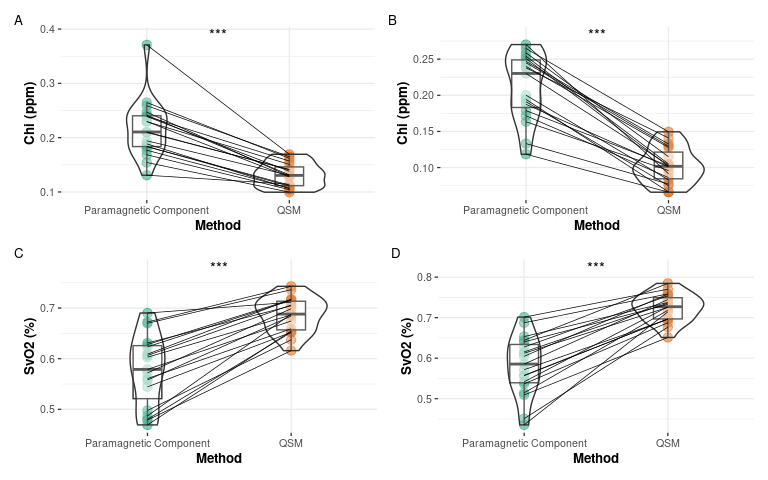
\includegraphics[keepaspectratio]{index_files/figure-latex/notebooks-gavin_thesis_markdown-fig-methodplot-output-1.png}}

}

\caption{\label{fig-methodplot}\textbf{Vein-specific susceptibility and
oxygen saturation values by method.} (A, B) contains violin plots
comparing subject chi (ppm) acquired from the cerebral central veins;
(C, D) contains violin plots comparing subject SvO2 (\%) acquired from
the superior sagittal sinus. Raw data points from paramagnetic maps are
shown as filled green circles and raw data points from QSM are shown as
filled orange circles. Each line connects the raw data points of a
single subject. (***) indicates P\textless0.05.}

\end{figure}%

\textsubscript{Source:
\href{https://WeberLab.github.io/Chisep_CSVO2_Manuscript/notebooks/gavin_thesis_markdown-preview.html\#cell-fig-methodplot}{gavin\_thesis\_R}}

The acquired \(\chi\) and SvO\textsubscript{2} values were additionally
compared between veins. In data created from QSM, a significant
difference was found between the CCV and SSS in mean \(\chi\) (p
\textless{} 0.05; 95\% CI {[}0.017, 0.04{]}) and mean
SvO\textsubscript{2} (p \textless{} 0.05; 95\% CI {[}-0.052, -0.023{]}).
In data acquired from paramagnetic maps, no significant difference was
observed between the CCV and the SSS in either mean \(\chi\) (p = 0.711;
95\% CI {[}-0.02, 0.029{]}) or mean SvO\textsubscript{2} (p = 0.752;
95\% CI {[}-0.034, 0.029{]}). A summary of these comparisons is
represented in Figure~\ref{fig-regionplot}.

\begin{figure}[H]

\centering{

\pandocbounded{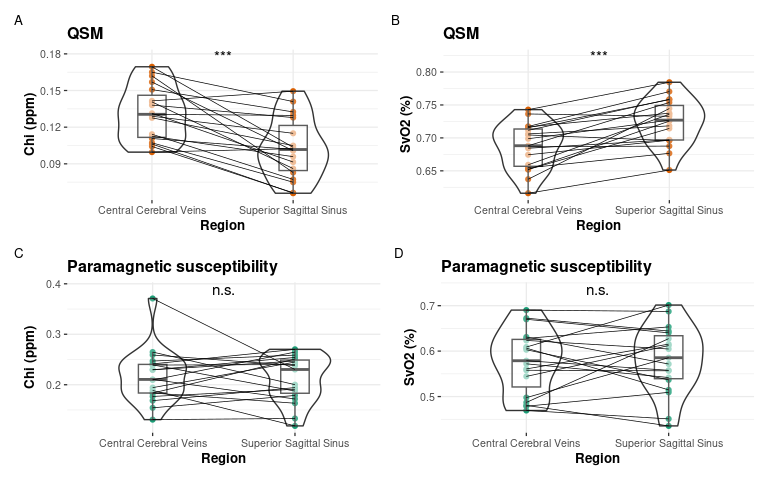
\includegraphics[keepaspectratio]{index_files/figure-latex/notebooks-gavin_thesis_markdown-fig-regionplot-output-1.png}}

}

\caption{\label{fig-regionplot}\textbf{Inter-venous comparisons of
susceptibility and oxygen saturation}. Violin plots comparing (A, C) chi
(ppm) and (B, D) SvO2 (\%) between the CCV and the SSS. Panels (A) and
(B) used data acquired from QSM, and its raw data points are shown as
filled orange circles. Panels (C) and (D) used data acquired from
paramagnetic maps, and its raw data points are shown as filled green
circles. Each line connects the raw data points of a single subject.
(***) indicates p\textless0.05; (n.s.) indicates no significant
difference.}

\end{figure}%

\textsubscript{Source:
\href{https://WeberLab.github.io/Chisep_CSVO2_Manuscript/notebooks/gavin_thesis_markdown-preview.html\#cell-fig-regionplot}{gavin\_thesis\_R}}

\section{Discussion}\label{sec-discussion}

The primary objective of the present study was to assess whether the
application of magnetic susceptibility separation to neonatal QSM data
could provide more accurate SvO\textsubscript{2} measurements without
the need for an arbitrary threshold value. To the best of our knowledge,
we are the first to test this in a neonatal cohort, as susceptibility
separation has been typically evaluated as a method of imaging myelin
and brain iron in adult subjects
\citep{shinHseparationMagneticSusceptibility2021, ahmedDiamagneticComponentMap2023a}.
Our results showed that the SvO\textsubscript{2} values of the SSS and
CCV obtained from susceptibility separation are significantly lower than
the respective SvO\textsubscript{2} values obtained from QSM alone. When
our results were compared to the literature (see below), we found that
our SSS SvO\textsubscript{2} data from susceptibility separation agreed
well with the findings of other studies measuring SvO\textsubscript{2}
of the SSS in similar subject populations. Conversely, the paramagnetic
CCV SvO\textsubscript{2} data saw less agreement with the existing
literature than the corresponding data from QSM. However, there is
reason to believe our paramagnetic CCV values may be accurate given
their similarity to the paramagnetic SSS values and the limitations of
the two studies that observed CCV SvO\textsubscript{2}. Additionally, it
is important to note that our SvO\textsubscript{2} measurements from
susceptibility separation had greater variance than our measurements
from QSM, indicating a limitation that should be addressed in future
research. Overall, the present work demonstrates the promise of
susceptibility separation as an MRI post-processing technique that can
measure the oxygenation of the cerebral veins of infant subjects, a
useful marker of regional oxygen consumption in the brain.

\subsection{Comparison with literature
values}\label{comparison-with-literature-values}

To evaluate the validity of our results, we compared the mean
SvO\textsubscript{2} values we obtained through QSM and susceptibility
separation to the mean SvO\textsubscript{2} values found by MRI studies
investigating the oxygenation of the SSS or the CCV. Notably, the number
of studies that measure the SvO\textsubscript{2} of the CCV, or any of
its individual veins, in infants is fairly lower than the number of
studies investigating the oxygenation of the SSS. Our comparison is
summarized in Table~\ref{tbl-litvalues}.

\begingroup\fontsize{9}{11}\selectfont

\begin{ThreePartTable}
\begin{TableNotes}[para]
\item PT-TEA = born preterm and scanned at term-equivalent age; late third trimester = >35 weeks gestational age; HIE = hypoxic-ischemic encephalopathy; TRUST = T2-relaxation-under-spin tagging; aTRUPC = accelerated T2-relaxation-under-phase-contrast; T2-TRIR = T2-tissue-relaxation-inversion-recovery; SWI = susceptibility weighted imaging.
\end{TableNotes}

\begin{longtable}[t]{ccllr}

\caption{\label{tbl-litvalues}\textbf{Cerebral oxygenation values of
neonates and fetuses in the literature.}}

\tabularnewline

\toprule
\textbf{Region} & \textbf{Study} & \textbf{Subjects} & \textbf{Method} & \textbf{SvO$_{2}$ (\%)}\\
\midrule
Whole-brain & \makecell[l]{Skov et al. \\(1993)    } & \makecell[l]{Preterm neonates \\(n=9)                   } & NIRS & 53.4 ± 15.4\\
Whole-brain & \makecell[l]{Skov et al. \\(1993)    } & \makecell[l]{Asphyxiated term \\neonates (n=10)           } & NIRS & 67.3 ± 9.4\\
Whole-brain & \makecell[l]{Altman et al. \\(1993)    } & \makecell[l]{Preterm and term \\neonates with HIE \\(n=11)} & PET & 21.6 ± 21.0\\
SSS & \makecell[l]{Gou et al. \\(2024)     } & \makecell[l]{Healthy neonates \\(n=37)                    } & \makecell[l]{MRI: \\TRUST   } & 66.7 ± 4.9\\
SSS & \makecell[l]{Jiang et al. \\(2019)   } & \makecell[l]{Healthy neonates \\(n=4)                     } & \makecell[l]{MRI: \\aTRUPC  } & 64.8 ± 2.9\\
SSS & \makecell[l]{De Vis et al. \\(2014)  } & \makecell[l]{PT-TEA \\neonates (n=18)                      } & \makecell[l]{MRI: \\T2-TRIR } & 52.0 ± 12.0\\
SSS & \makecell[l]{Yadav et al. \\(2020)} & \makecell[l]{Late third \\trimester fetuses \\(n=33)} & \makecell[l]{MRI: \\Susceptometry} & 58.6 ± 4.8\\
SSS & \textbf{This study} & \makecell[l]{PT-TEA \\neonates \\n=19} & \makecell[l]{MRI: \\QSM} & 72.46 ± 3.43\\
SSS & \textbf{This study} & \makecell[l]{PT-TEA \\neonates \\n=19} & \makecell[l]{MRI: \\ χ-separation} & 58.14 ± 7.3\\
CCV & Weber et al. (2021) & \makecell[l]{Preterm neonates \\with HIE (n=8)} & \makecell[l]{MRI: \\QSM} & 72.2 ± 6.0\\
CCV & Weber et al. (2021) & \makecell[l]{Healthy neonates \\(n=8)} & \makecell[l]{MRI: \\QSM} & 73.6 ± 2.8\\
CCV & Jiang et al. (2019) & \makecell[l]{Healthy neonates \\(n=4)} & \makecell[l]{MRI: \\aTRUPC} & 70.2 ± 3.3\\
CCV & \textbf{This study} & \makecell[l]{PT-TEA \\neonates \\n=19} & \makecell[l]{MRI: \\QSM} & 68.71 ± 0.03\\
CCV & \textbf{This study} & \makecell[l]{PT-TEA \\neonates \\n=19} & \makecell[l]{MRI: \\ χ-separation} & 57.69 ± 6.97\\
\bottomrule
\insertTableNotes

\end{longtable}

\end{ThreePartTable}
\endgroup{}

\textsubscript{Source:
\href{https://WeberLab.github.io/Chisep_CSVO2_Manuscript/index.qmd.html}{Article
Notebook}}

As shown in Table~\ref{tbl-litvalues}, the infants observed in MRI
studies investigating cerebral vein oxygenation noticeably differ in
clinical status, with three studies involving healthy neonates
\citep{weberQuantitativeSusceptibilityMapping2021, gouAutomaticRejectionBased2024, jiangVesselspecificQuantificationNeonatal2019},
three studies (including the present study) involving preterm neonates
\citep{weberQuantitativeSusceptibilityMapping2021, devisNoninvasiveMRIMeasurements2014},
and one study involving late third trimester fetuses
\citep{portnoyHumanUmbilicalCord2018}. In the studies involving healthy
neonates, the SvO\textsubscript{2} of the SSS fell within the range of
64.8\% -- 66.6\%
\citep{gouAutomaticRejectionBased2024, jiangVesselspecificQuantificationNeonatal2019},
while the SvO\textsubscript{2} of the CCV fell within the range of
70.2\% - 73.6\%
\citep{weberQuantitativeSusceptibilityMapping2021, jiangVesselspecificQuantificationNeonatal2019}.
Notably, the SvO\textsubscript{2} value of the SSS we obtained from
susceptibility separation (58.14\%) was closest to values obtained from
the studies involving late third trimester fetuses
\citep{yadavImagingPutativeFoetal2018} or pre-term neonates
\citep{devisNoninvasiveMRIMeasurements2014}, each finding an SSS
SvO\textsubscript{2} value of 58.6\% and 52.0\%, respectively. It is
important to note the difference in MRI modalities used to obtain these
values. For their study, \citet{yadavImagingPutativeFoetal2018} used MR
susceptometry, which involves measuring the difference in phase between
the chosen vessel and its background in imaging data from an SWI
scanning sequence \citep{yadavImagingPutativeFoetal2018}. In
\citet{devisNoninvasiveMRIMeasurements2014}, the authors used T2-TRIR,
which allowed them to determine the transverse relaxation rate of blood
within the vessel, which can be used alongside hematocrit data to
estimate SvO\textsubscript{2}. Additionally, the GA of infants scanned
in our study ranged between 37 and 44 weeks, while the GA of the fetuses
scanned in \citet{yadavImagingPutativeFoetal2018} was ≥35 weeks and the
GA of infants scanned in \citet{devisNoninvasiveMRIMeasurements2014}
ranged between 38 and 40 weeks. As such, our SSS SvO\textsubscript{2}
values found through susceptibility separation show promise given their
similarity to the SvO\textsubscript{2} values found by
\citet{yadavImagingPutativeFoetal2018} and
\citet{devisNoninvasiveMRIMeasurements2014}, two studies that involved
comparable subject populations and used considerably different methods.

Conversely, the SvO\textsubscript{2} value of the CCV we obtained
through QSM (68.71\%) was closest to values from similar studies in the
literature. In \citet{weberQuantitativeSusceptibilityMapping2021}, QSM
was used to measure an SvO\textsubscript{2} of 71.5\% in preterm
neonates with HIE and an SvO\textsubscript{2} of 73.6\% in healthy
neonates. In their study,
\citet{jiangVesselspecificQuantificationNeonatal2019} also involved
healthy neonates and obtained an SvO\textsubscript{2} of 70.2\% through
an accelerated TRUPC sequence. In contrast, the SvO\textsubscript{2} of
the CCV we obtained through susceptibility separation was 57.69\%. This
disparity from the literature, however, may not undermine the value we
obtained, as the study design of
\citet{weberQuantitativeSusceptibilityMapping2021} and
\citet{jiangVesselspecificQuantificationNeonatal2019} may prevent their
values from being representative of the study demographic. In
\citet{weberQuantitativeSusceptibilityMapping2021}, the authors utilized
an arbitrary 0.15 ppm threshold and included all \(\chi\) values above
0.15 when measuring the mean \(\chi\) of the CCV, which potentially led
to the introduction of \(\chi\) from veins outside the CCV. In
\citet{jiangVesselspecificQuantificationNeonatal2019}, the authors
acquired their data from 4 subjects, a notably small sample size. Given
the limitations of the existing literature and the similarity of the
mean paramagnetic CCV SvO\textsubscript{2} value (57.69\%) to the mean
paramagnetic SSS SvO\textsubscript{2} value (58.14\%), it is plausible
that susceptibility separation provides more accurate measurements of
oxygenation in both cortical and subcortical veins. One reason for this
is due to its ability to mitigate partial volume effects, which are
likely to contaminate other methods resulting in inaccurate
CSvO\textsubscript{2} values
\citep{shinHseparationMagneticSusceptibility2021}.

Another notable distinction between our findings and those of the
existing literature was that we observed no significant oxygenation
difference between the SSS and the CCV when \(\chi\) was derived from
paramagnetic maps.
\citet{jiangVesselspecificQuantificationNeonatal2019}, the only other
study that also measured SvO\textsubscript{2} in both the SSS and CCV,
observed significantly lower oxygenation in the SSS (64.8\%) when
compared to the CCV (70.2\%). Given the small sample size utilized by
\citet{jiangVesselspecificQuantificationNeonatal2019}, it is difficult
to ascertain whether this is generalizable to all neonates.

\subsection{Limitations and future
directions}\label{limitations-and-future-directions}

This study has a few limitations that should be considered for future
research. Firstly, only 19 infants were recruited for scanning. Given
the emotional toll placed on parents when their child is born preterm,
it is understandable that they may show reluctance in consenting to
further testing that is not medically necessary. Obtaining a larger
sample size in future studies, however, may provide greater insight into
the efficacy of susceptibility separation. Secondly, this study did not
include healthy neonates born at term, resulting in a lack of a control
cohort. This is because recruiting healthy controls when there is no
contraindication is very difficult. The addition of such a group may
provide further validity to any findings and may reveal potential
differences in cerebral oxygen consumption between term and preterm
neonates. Finally, future studies should consider the use of multi-echo
T2 imaging data when performing the decomposition of QSM images. The
toolbox applied by this study for QSM decomposition
\citep{shinHseparationMagneticSusceptibility2021} utilizes R2 data,
which can be obtained from multi-echo T2 imaging. Our study protocol
involved the collection of multi-echo SWI imaging data, and as such, we
could only use R2\textsuperscript{*} data to perform the decomposition.
Furthermore, this may account for the reduced precision of
SvO\textsubscript{2} values obtained through susceptibility separation.

\section{Conclusion}\label{sec-conclusion}

This study aimed to evaluate how the use of susceptibility separation on
preterm neonatal QSM images could be used in determining the oxygenation
of cerebral venous vessels. We compared venous specific
SvO\textsubscript{2} values obtained from QSM images and their
respective paramagnetic components to SvO\textsubscript{2} values from
neonatal MRI studies. We found that susceptibility separation provided
SvO\textsubscript{2} values of the SSS that were comparable to values
found in the literature, providing evidence that this processing
technique may be a valid tool for measuring regional cerebral oxygen
consumption. Additionally, we were able to simultaneously measure
SvO\textsubscript{2} in both the SSS and CCV, which permitted us to
observe no difference in oxygenation between the two vessels when
considering data from isolated paramagnetic components. Ultimately, we
hope our work inspires future studies that seek to explore and improve
the capabilities of magnetic susceptibility separation, culminating in
the development of a tool for clinicians and researchers alike.

\newpage{}

\subsection{Data availability}\label{data-availability}

The manuscript was written in a `reproducible manner'. The entire
manuscript, including statistics reported, figures, and tables, can be
reproduced here:
\href{https://weberlab.github.io/Chisep_CSVO2_Manuscript}{weberlab.github.io/Chisep\_CSVO2\_Manuscript}

Unfortunately, we can not upload our MRI images to an open repository as
we did not obtain permission in our consent forms.

\section*{References}\label{references}
\addcontentsline{toc}{section}{References}

\renewcommand{\bibsection}{}
\bibliography{Gavin_Thesis_Ref.bib}

\subsection{Acknowledgments}\label{acknowledgments}

We wish to acknowledge the work of and thank Victoria Tapics (Research
Nurse); Vicki Goh (Research Nurse); Chacko Anil (Neonatologist); and
Michael A. Sargent (Radiologist).

\subsection{Author contributions}\label{author-contributions}

TGC wrote the original draft, performed the formal analysis, and
contributed to methodology, validation, and visualization. AR helped
with writing, reviewing \& editing. REG helped with writing, reviewing
\& editing, and with initial funding acquisition. AMW was involved in
project administration, supervision, validation, visualization,
resources, methodology, formal analysis, funding acquisition, writing,
reviewing \& editing, conceptualization, data curation, and
investigation.

\subsection{Funding}\label{funding}

Authors AMW and REG were co-primary applicants for a BC Children's
Hospital Research Institute - Brain, Behaviour and Development Catalyst
Grant (\$20,000). AMW was supported by an establishment award from
BCCHRI. Scanning was partly funded through a special award to AMW from
BCCHRI .

\subsection{Competing interests}\label{competing-interests}

The authors have no competing interests to declare.

\subsection{Consent statement}\label{consent-statement}

The study was approved by the Clinical Research Ethics Board at the
University of British Columbia and Children's \& Women's Hospital
(H21-00655) and written informed consent was obtained from the
parent/guardian for each infant.





\end{document}
